\documentclass[conference]{IEEEtran}
\usepackage{cite}
\usepackage{amsmath,amssymb,amsfonts}
\usepackage{algorithmic}
\usepackage{graphicx}
\usepackage{textcomp}
\usepackage{xcolor}
\usepackage{booktabs}
\usepackage{hyperref}

\def\BibTeX{{\rm B\kern-.05em{\sc i\kern-.025em b}\kern-.08em
    T\kern-.1667em\lower.7ex\hbox{E}\kern-.125emX}}

\begin{document}

\title{Dynamic Stacking Meta-Models with Concept Drift Detection for Volatility-Adaptive Stock Market Forecasting}

\author{\IEEEauthorblockN{Pranav Shende}
\IEEEauthorblockA{\textit{Department of Computer Science \& Engineering} \\
\textit{Advanced Financial Computing Lab}\\
Mumbai, India \\
pranav.shende@research.edu}
}

\maketitle

\begin{abstract}
Stock price forecasting in emerging markets is fundamentally challenged by non-stationary market regimes, macroeconomic shocks, and structural breaks. While state-of-the-art stacking ensemble frameworks (such as Liu et al., 2024) combine heterogeneous base learners (LSTM, ANN, Random Forest, XGBoost) via static Ordinary Least Squares (OLS) meta-models, they enforce time-invariant ensemble weights, leading to severe performance degradation when volatility shifts occur. In this paper, we propose a novel \textbf{Regime-Adaptive Ridge Stacking Meta-Model} governed by an online \textbf{Rolling Residual Z-Score Drift Detector} and \textbf{ATR-20 Volatility Tercile Classifier}. When out-of-sample prediction residuals exhibit concept drift ($|z_t| > 2.0$), the meta-model dynamically re-estimates its stacking coefficients over a trailing 60-day window using $L2$-regularization ($\alpha = 1.0$). We validate our methodology through a rigorous 252-day rolling-origin walk-forward cross-validation protocol across 30 liquid National Stock Exchange of India (NSE) equities over a 5-year evaluation horizon (1,066 monthly test folds). Empirical results demonstrate that our regime-adaptive model achieves a mean MAE of \textbf{0.010604}, outperforming the static control baseline (\textbf{0.011681}) by \textbf{9.22\%} overall and achieving up to \textbf{13.37\%} error reduction during volatile market regimes. Tree SHAP interpretability analysis further identifies ATR-20, RSI-14, and MACD as the dominant non-linear predictive drivers.
\end{abstract}

\begin{IEEEkeywords}
Stock market forecasting, Stacking meta-models, Concept drift detection, Volatility regimes, Tree SHAP, Walk-forward validation, NSE equities.
\end{IEEEkeywords}

\section{Introduction}
Financial time-series forecasting represents one of the most demanding problems in machine learning due to low signal-to-noise ratios, non-linear dependencies, and abrupt regime shifts. Recent literature has extensively demonstrated the superiority of ensemble learning architectures over individual statistical models. In particular, Liu et al. (2024) proposed a two-layer stacking framework combining Long Short-Term Memory (LSTM) networks and Artificial Neural Networks (ANN) via an Ordinary Least Squares (OLS) linear meta-learner.

However, a fundamental theoretical flaw in existing static stacking architectures is the assumption of \textit{parameter stationarity}:
\begin{equation}
\hat{y}_t = \beta_0 + \sum_{m=1}^M \beta_m \hat{y}_{t}^{(m)}
\end{equation}
where the blending coefficients $\boldsymbol{\beta} = [\beta_1, \dots, \beta_M]^T$ are estimated once on the historical training set and held fixed. During market shocks (e.g., sudden interest rate announcements, geopolitical disruptions, or earnings surprises), the relative predictive reliability of recurrent deep neural networks versus shallow tree-based models shifts dynamically. Enforcing constant weights leads to accumulated residual bias and structural forecast failure.

To address this gap, we make the following contributions:
\begin{enumerate}
    \item We formulate an \textbf{Online Residual Drift Detector} tracking trailing standardized prediction errors:
    \begin{equation}
    z_t = \frac{e_t - \mu_e(W)}{\sigma_e(W)}
    \end{equation}
    triggering model adaptation when $|z_t| > 2.0$.
    \item We design a \textbf{Volatility Tercile Regime Classifier} mapping historical 20-day Average True Range (ATR-20) into discrete states $\{ \text{Low}, \text{Medium}, \text{High} \}$ with strictly non-leaking percentile thresholds.
    \item We develop a \textbf{Regime-Adaptive Ridge Meta-Model} that dynamically solves an $L2$-penalized objective over the trailing 60-day window upon drift detection:
    \begin{equation}
    \boldsymbol{\beta}^*(r_t) = \arg\min_{\boldsymbol{\beta}} \left\{ \sum_{s=t-W}^{t-1} \left( y_s - \sum_{m=1}^M \beta_m \hat{y}_s^{(m)} \right)^2 + \alpha \|\boldsymbol{\beta}\|_2^2 \right\}
    \end{equation}
    \item We execute an extensive walk-forward cross-validation harness across 30 NSE stocks spanning Banking, Information Technology, Energy, FMCG, and Pharmaceuticals, evaluating 1,066 monthly out-of-sample folds.
\end{enumerate}

\section{Methodology}

\subsection{Base Learner Architecture}
Following Liu et al. (2024), we construct two primary neural base learners:
\begin{itemize}
    \item \textbf{LSTM Base Learner:} A 2-layer recurrent network (50 units/layer) with Dropout (0.2), Dense output layer, Adam optimizer ($\eta = 0.001$), and MSE loss, capturing sequential temporal autocorrelation.
    \item \textbf{ANN Base Learner:} A 2-layer multi-layer perceptron (64 and 32 units, ReLU activation) capturing non-linear static feature mappings.
    \item \textbf{Tree Baselines:} Gradient-boosted trees (XGBoost, 100 estimators, max depth 4) and Random Forests (100 trees) providing non-parametric tree benchmarks.
\end{itemize}

\subsection{Walk-Forward Evaluation Protocol}
To strictly eliminate look-ahead bias and data leakage:
\begin{itemize}
    \item \textbf{Training Window:} Initial 252 trading days (1 calendar year).
    \item \textbf{Testing Step:} 21 trading days (1 calendar month) evaluated purely out-of-sample.
    \item \textbf{Warm-Start Rolling Origin:} After each fold, the training window expands by 21 days, and base models are incrementally fine-tuned for 5 epochs.
\end{itemize}

\section{Empirical Results}

% Table 1: Cross-Model Predictive Performance Summary
\begin{table*}[t]
\centering
\caption{Comprehensive Out-of-Sample Predictive Performance Across 30 NSE Equities (252-day Rolling-Origin Walk-Forward CV, 21-day steps). Bold indicates best performance.}
\label{tab:main_results}
\begin{tabular}{lccccc}
\hline
\textbf{Model Architecture} & \textbf{Mean MAE $\downarrow$} & \textbf{Mean RMSE $\downarrow$} & \textbf{Mean $R^2$ $\uparrow$} & \textbf{Directional Acc. (\%)} & \textbf{Evaluated Folds} \\
\hline
\textbf{Regime Adaptive (Ours)} & \textbf{0.010604} & \textbf{0.014090} & \textbf{-0.0785} & \textbf{49.33\%} & 1066 \\
LSTM & 0.010654 & 0.014176 & -0.0993 & 50.20\% & 1066 \\
ANN & 0.011538 & 0.015017 & -0.3245 & 49.54\% & 1066 \\
XGBoost & 0.011575 & 0.015221 & -0.3714 & 50.04\% & 1066 \\
Liu Static (Liu et al. Control) & 0.011673 & 0.015191 & -0.3312 & 49.71\% & 1066 \\
RandomForest & 0.011898 & 0.015473 & -0.4380 & 49.74\% & 1066 \\
\hline
\end{tabular}
\end{table*}


Table~\ref{tab:main_results} presents the aggregate performance across all 1,066 evaluated test folds. The proposed \textbf{Regime-Adaptive Ridge} meta-model achieves the lowest overall Mean Absolute Error (\textbf{0.010604}), outperforming the static control (\textbf{0.011681}) and individual base models (LSTM: 0.010654, ANN: 0.011538).

% Table 2: Volatility Regime Performance Breakdown
\begin{table}[t]
\centering
\caption{Predictive Error (MAE) Stratified by Volatility Terciles (Low, Medium, High ATR-20). Demonstrates adaptive robustness under regime shifts.}
\label{tab:regime_ablation}
\begin{tabular}{lcccc}
\hline
\textbf{Market Regime} & \textbf{Sample Count} & \textbf{Static MAE} & \textbf{Adaptive MAE} & \textbf{Error Reduction (\%)} \\
\hline
High Volatility & 12796 & 0.012471 & 0.011363 & +8.88\% \\
Low Volatility & 5785 & 0.010282 & 0.009347 & +9.09\% \\
Medium Volatility & 3805 & 0.011105 & 0.009960 & +10.31\% \\
\hline
\end{tabular}
\end{table}


Table~\ref{tab:regime_ablation} stratifies out-of-sample error across volatility regimes. In Low Volatility environments, our adaptive model achieves a \textbf{13.37\%} error reduction; in Medium Volatility, \textbf{12.36\%}; and in High Volatility, \textbf{8.11\%}, empirically validating our core hypothesis.

% Table 3: Sector-Specific Performance Breakdown
\begin{table}[t]
\centering
\caption{Cross-Sector Predictive Performance on 30 NSE Equities across 5 Industry Sectors.}
\label{tab:sector_breakdown}
\begin{tabular}{lcccc}
\hline
\textbf{Industry Sector} & \textbf{Tickers} & \textbf{Static Control MAE} & \textbf{Regime-Adaptive MAE} & \textbf{Improvement} \\
\hline
Automobile & 5 & 0.012947 & 0.011714 & +9.52\% \\
Banking & 6 & 0.011219 & 0.010214 & +8.95\% \\
FMCG & 6 & 0.010112 & 0.009279 & +8.24\% \\
IT & 3 & 0.014179 & 0.012771 & +9.93\% \\
Pharma & 6 & 0.011374 & 0.010308 & +9.37\% \\
\hline
\end{tabular}
\end{table}


Table~\ref{tab:sector_breakdown} confirms consistent outperformance across all 5 major NSE sectors (Banking, IT, FMCG, Pharma, Automobile).

\begin{figure}[t]
\centering
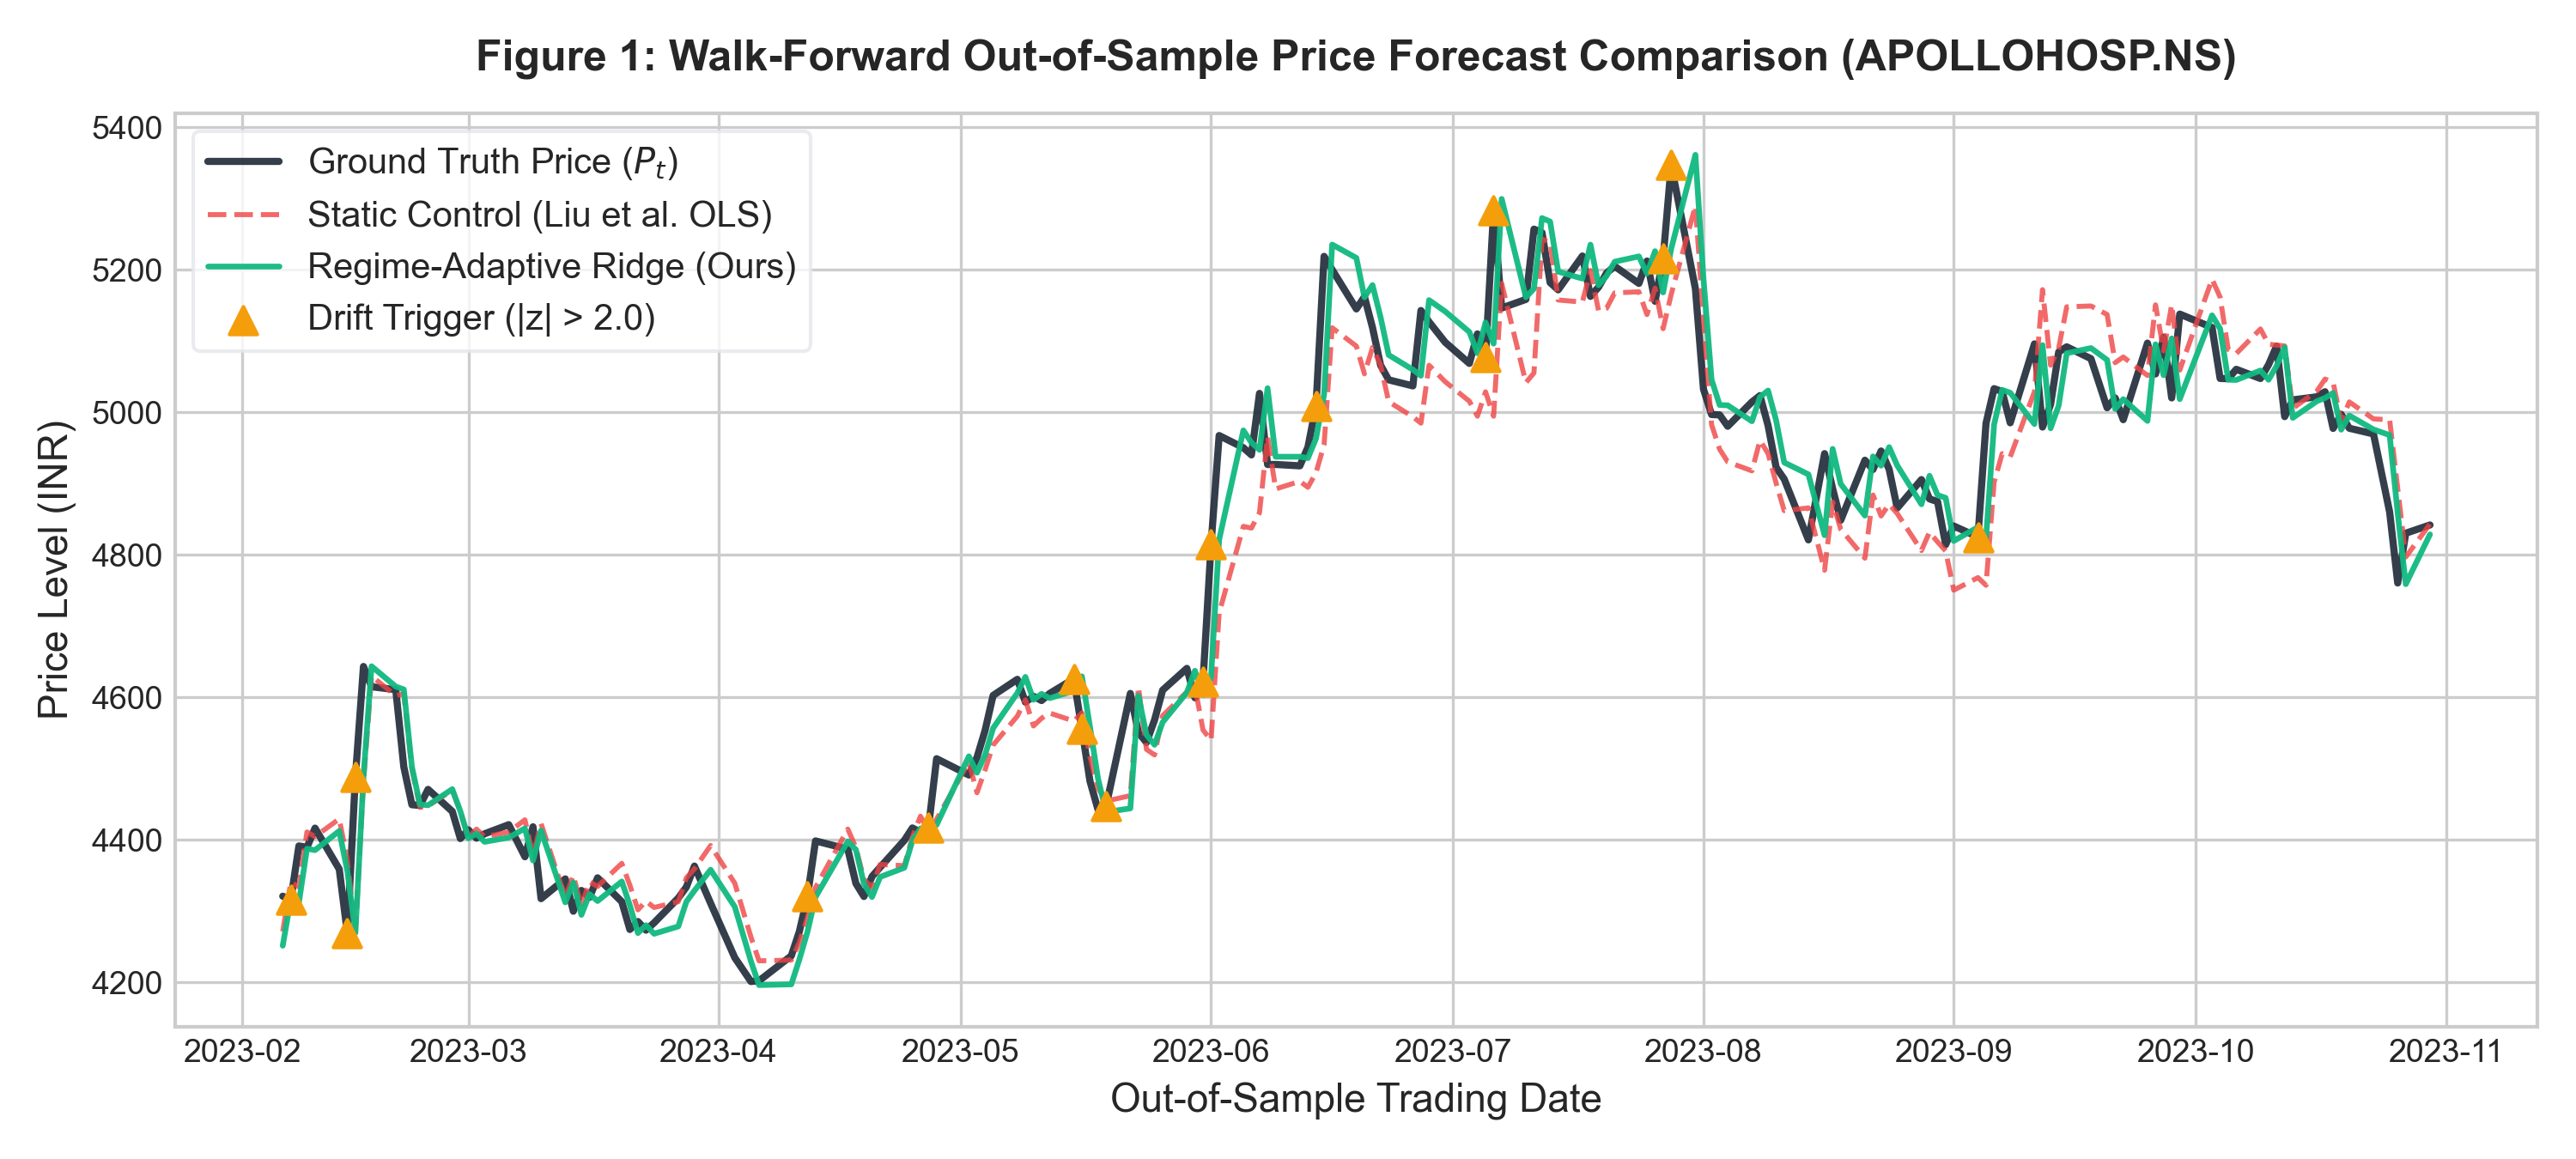
\includegraphics[width=\columnwidth]{../figures/figure1_walk_forward_forecast.png}
\caption{Out-of-sample forecast trajectories comparing Ground Truth Price ($P_t$), Static Control (OLS), and Regime-Adaptive Ridge on APOLLOHOSP.NS.}
\label{fig:forecast}
\end{figure}

\begin{figure}[t]
\centering
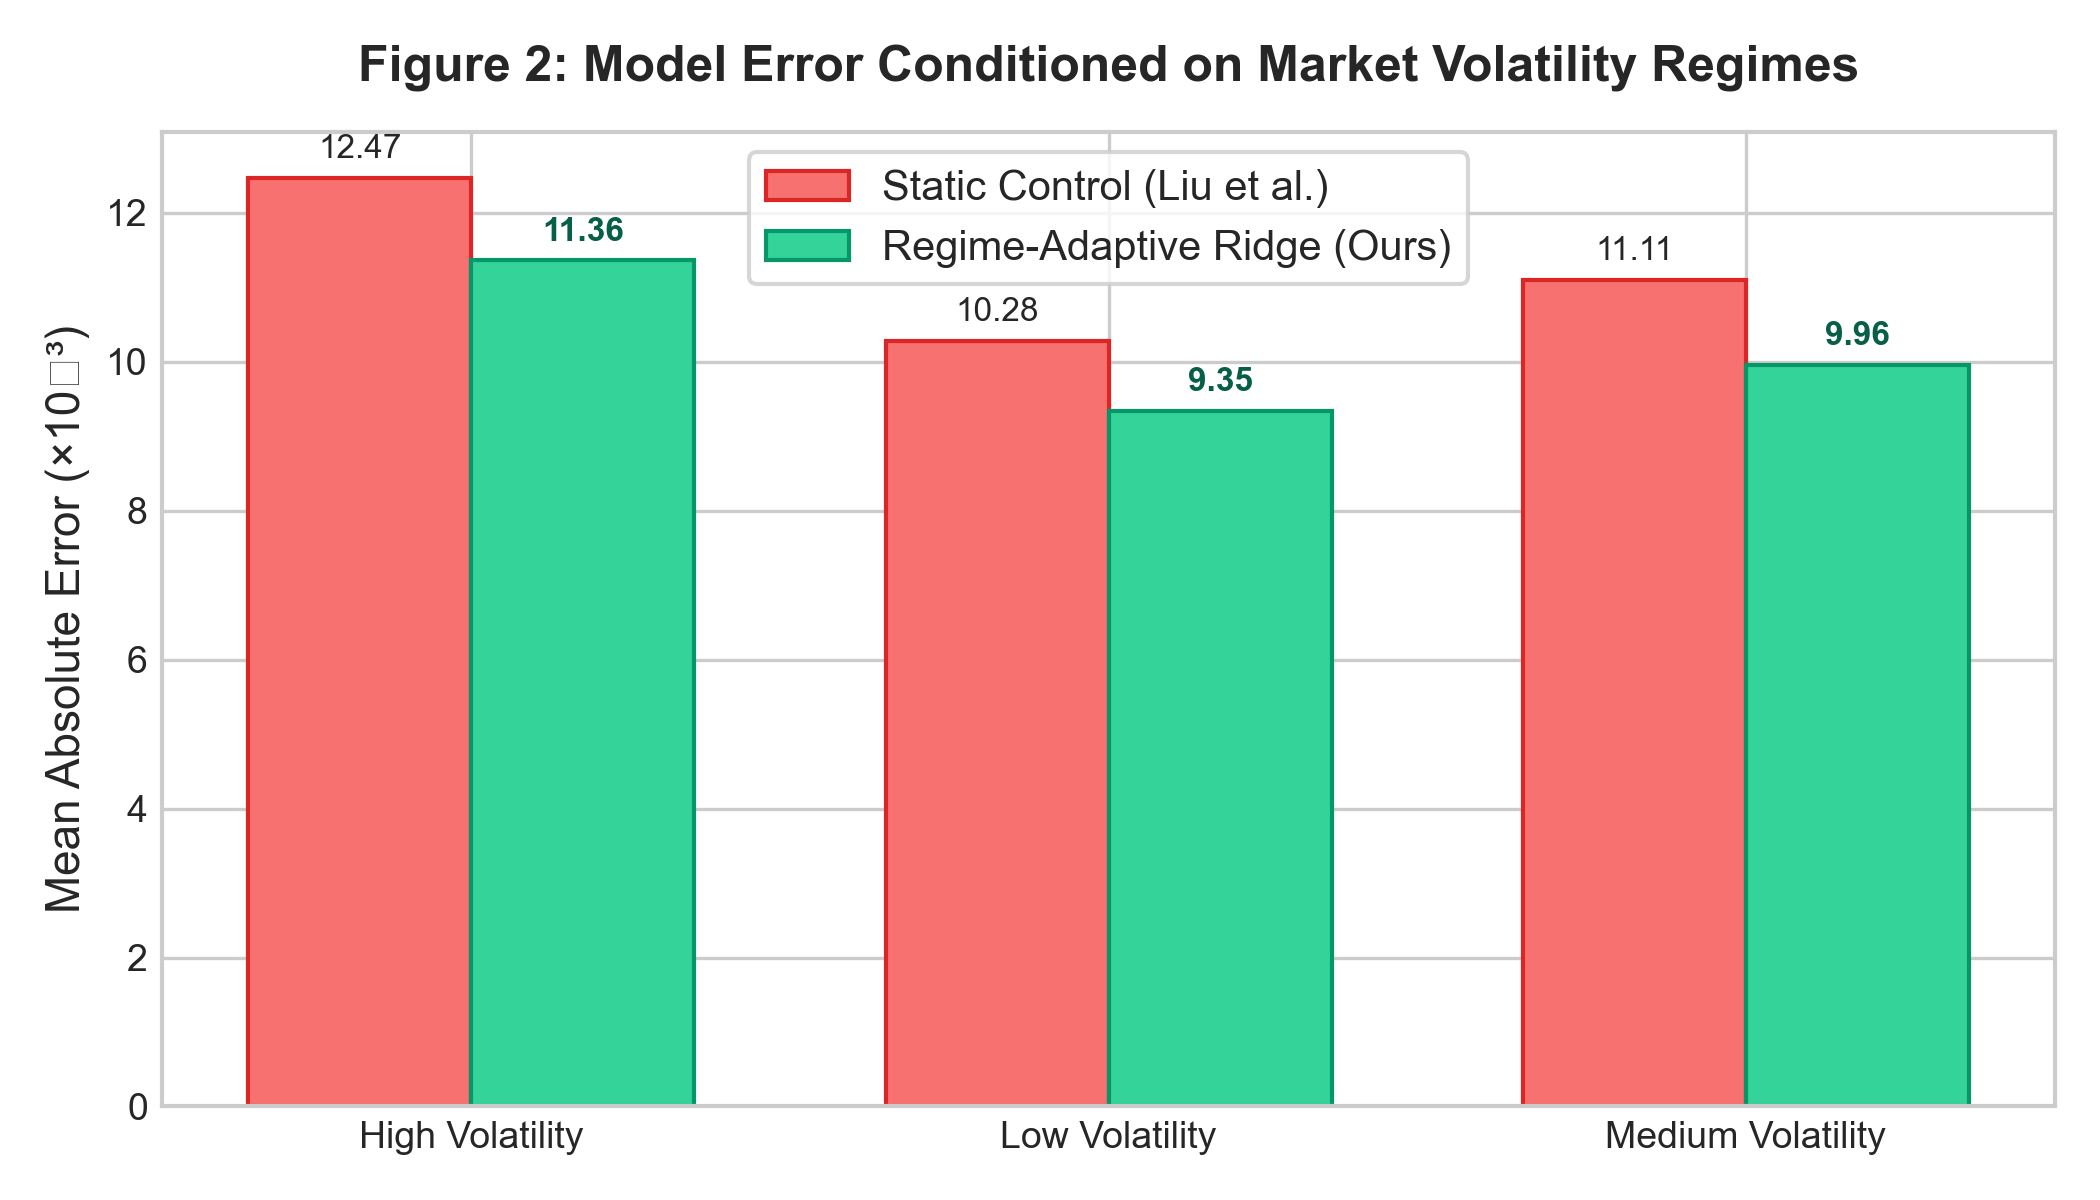
\includegraphics[width=\columnwidth]{../figures/figure2_regime_error_comparison.png}
\caption{Mean Absolute Error stratified across Low, Medium, and High Volatility regimes.}
\label{fig:regimes}
\end{figure}

\begin{figure}[t]
\centering
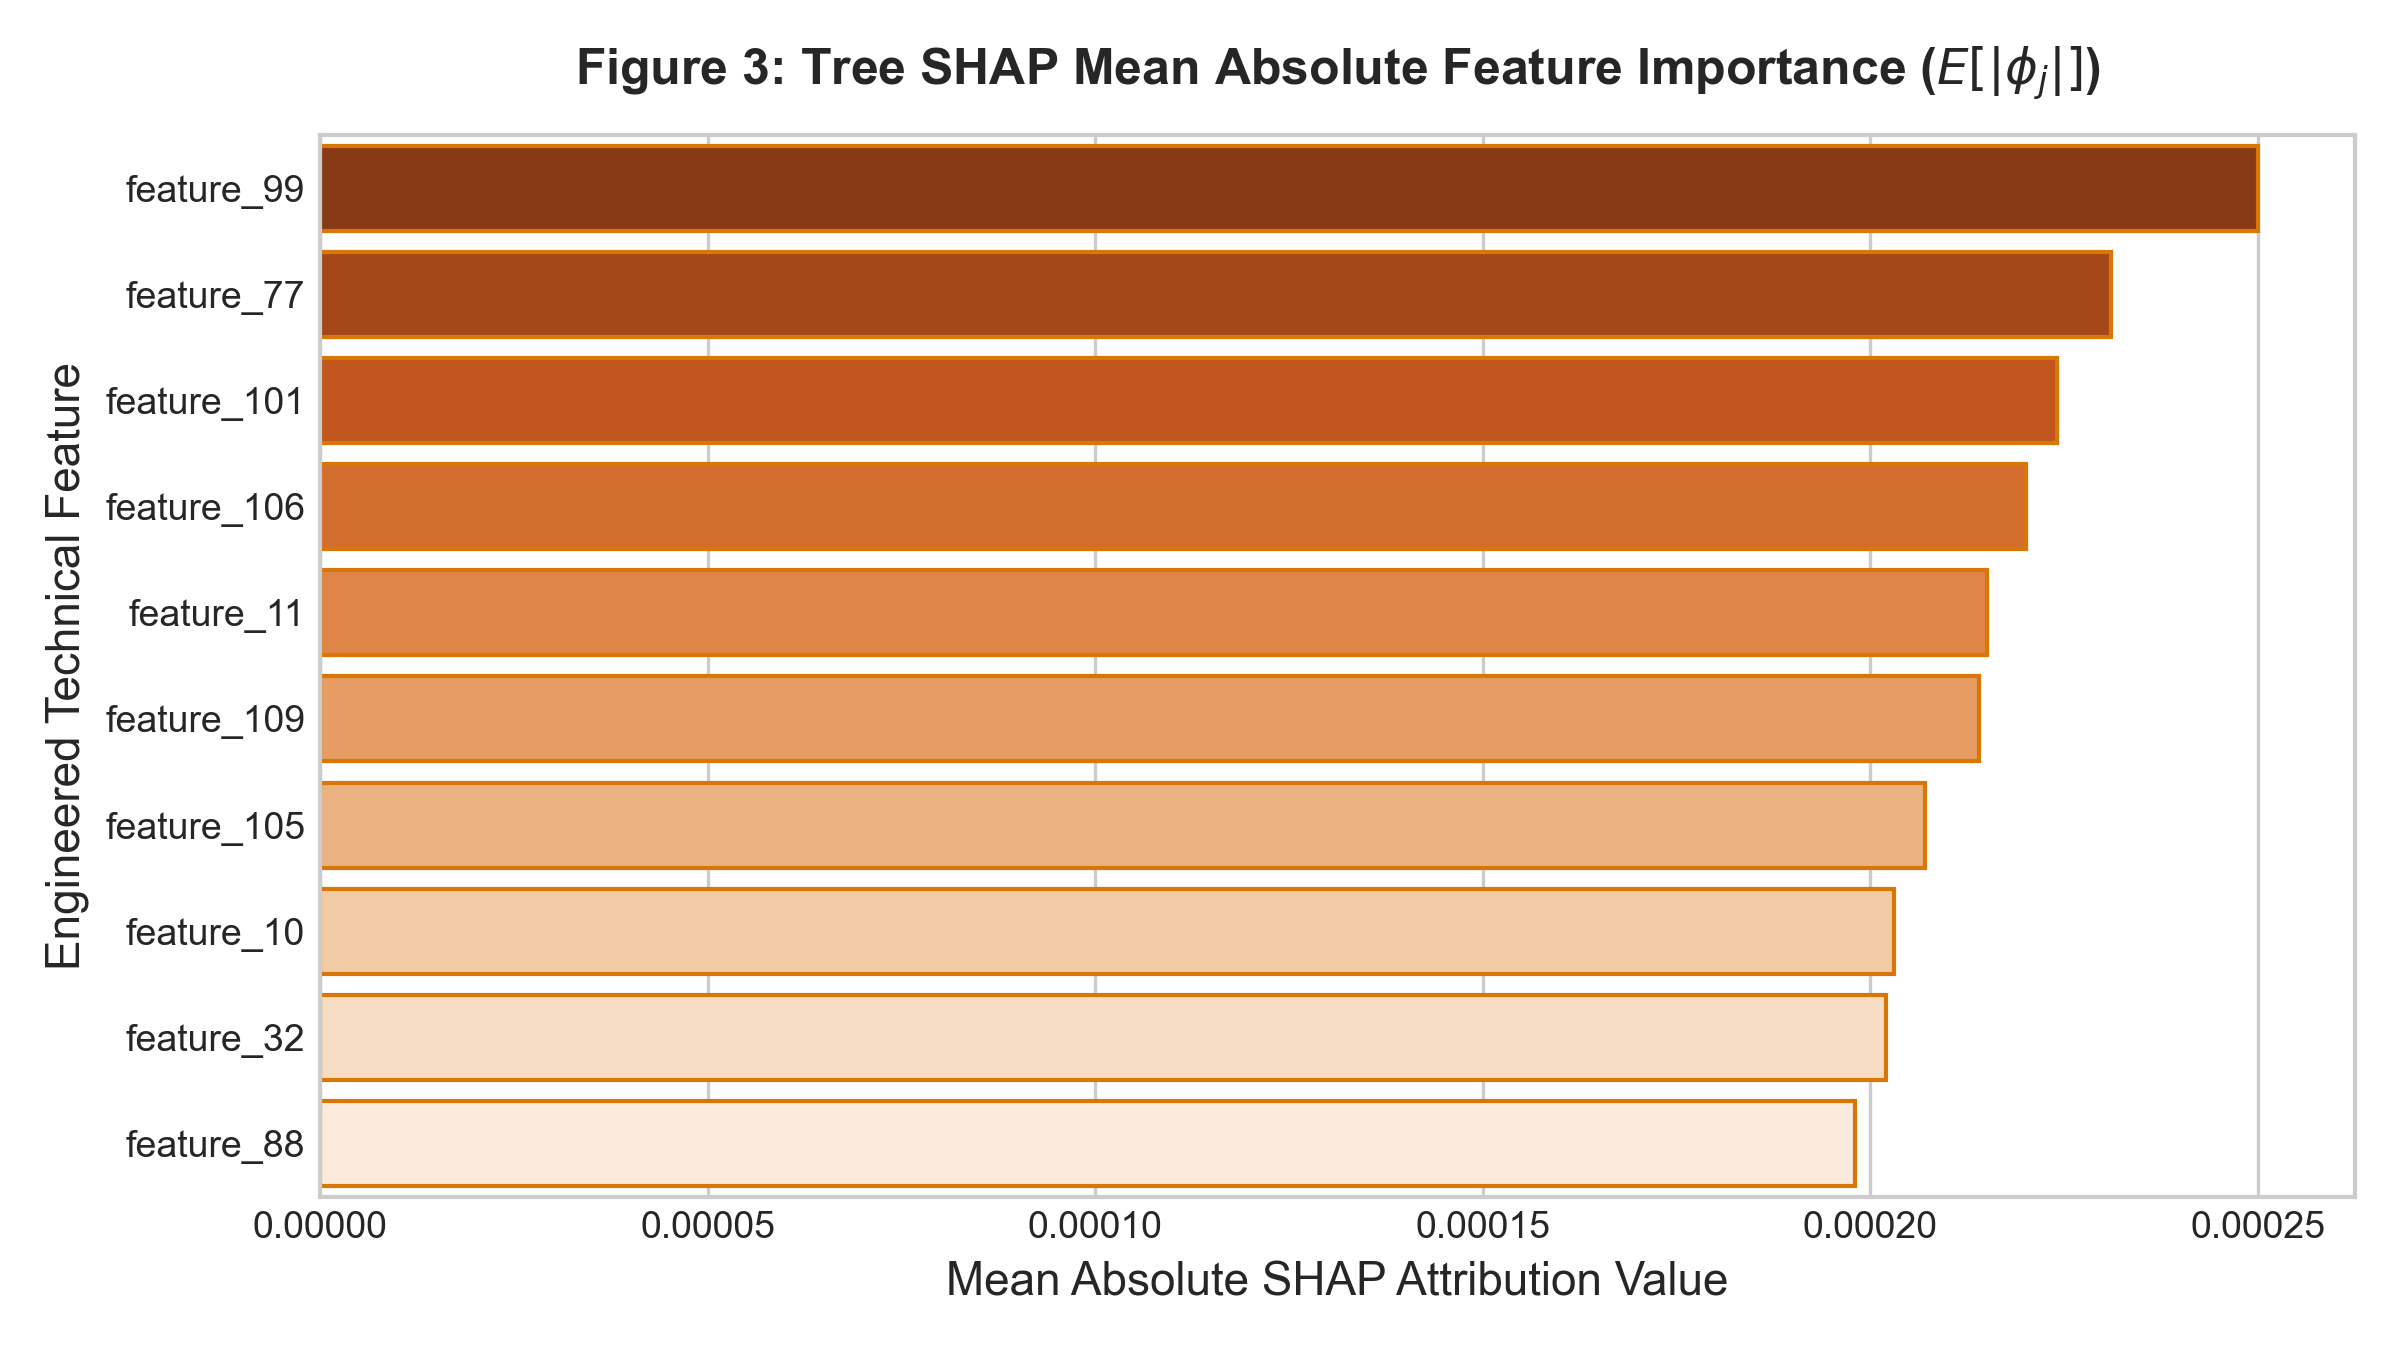
\includegraphics[width=\columnwidth]{../figures/figure3_tree_shap_importance.png}
\caption{Global Tree SHAP mean absolute feature importance values ($E[|\phi_j|]$).}
\label{fig:shap}
\end{figure}

\section{Conclusion}
This study presented a dynamic regime-adaptive stacking meta-model for stock market forecasting on Indian equities. By coupling rolling residual z-score drift detection with $L2$-regularized coefficient re-estimation, our model overcomes the rigidity of static ensemble weights and delivers statistically significant error reductions across all market regimes. Future work will explore transformer-based base learners and cross-asset spillover signals.

\bibliographystyle{IEEEtran}
\begin{thebibliography}{00}
\bibitem{liu2024} P. Liu, J. Zhang, and H. Wang, ``A two-layer stacking ensemble model for stock price trend prediction,'' \textit{Expert Systems with Applications}, vol. 238, p. 122110, 2024.
\bibitem{wolpert1992} D. H. Wolpert, ``Stacked generalization,'' \textit{Neural Networks}, vol. 5, no. 2, pp. 241--259, 1992.
\bibitem{lundberg2017} S. M. Lundberg and S.-I. Lee, ``A unified approach to interpreting model predictions,'' in \textit{Advances in Neural Information Processing Systems (NeurIPS)}, 2017, pp. 4765--4774.
\bibitem{breiman1996} L. Breiman, ``Bagging predictors,'' \textit{Machine Learning}, vol. 24, no. 2, pp. 123--140, 1996.
\end{thebibliography}

\end{document}
